\chapter{Conclusion}
The complete workflow consists of FPGA Implementation and scheduler mentioned is given in the following figure:-


\begin{figure}[H]
    \centering
    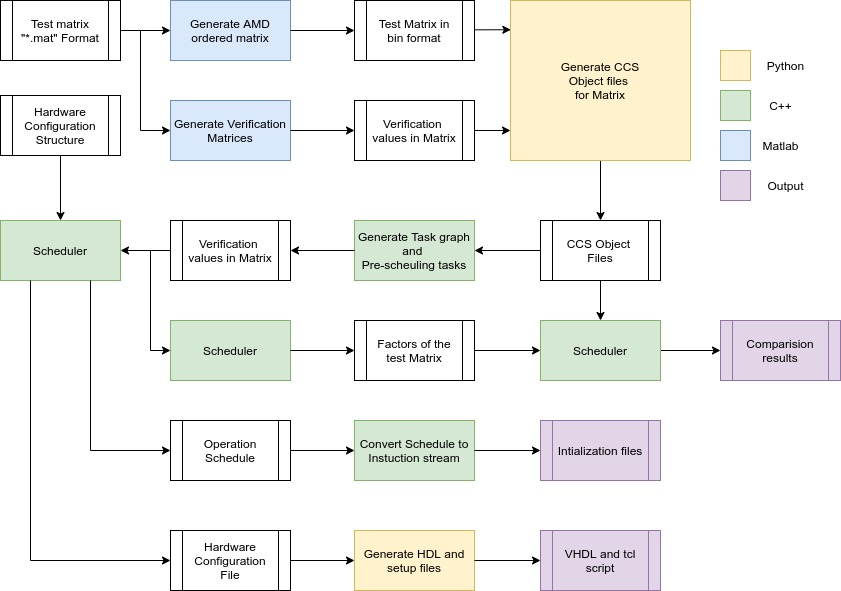
\includegraphics[width = \textwidth]{./Software/Workflow.jpg}
    \caption{Workflow of Software}
\end{figure}


The hardware is generated to an AXI wrapper IP such that it can be connectable with the Microblaze (soft-core processor)  or  ZynQ (hard-core processor) is generated. The following is the report of Dual Port IP hardware.\\



\begin{figure}[H]
    \centering
    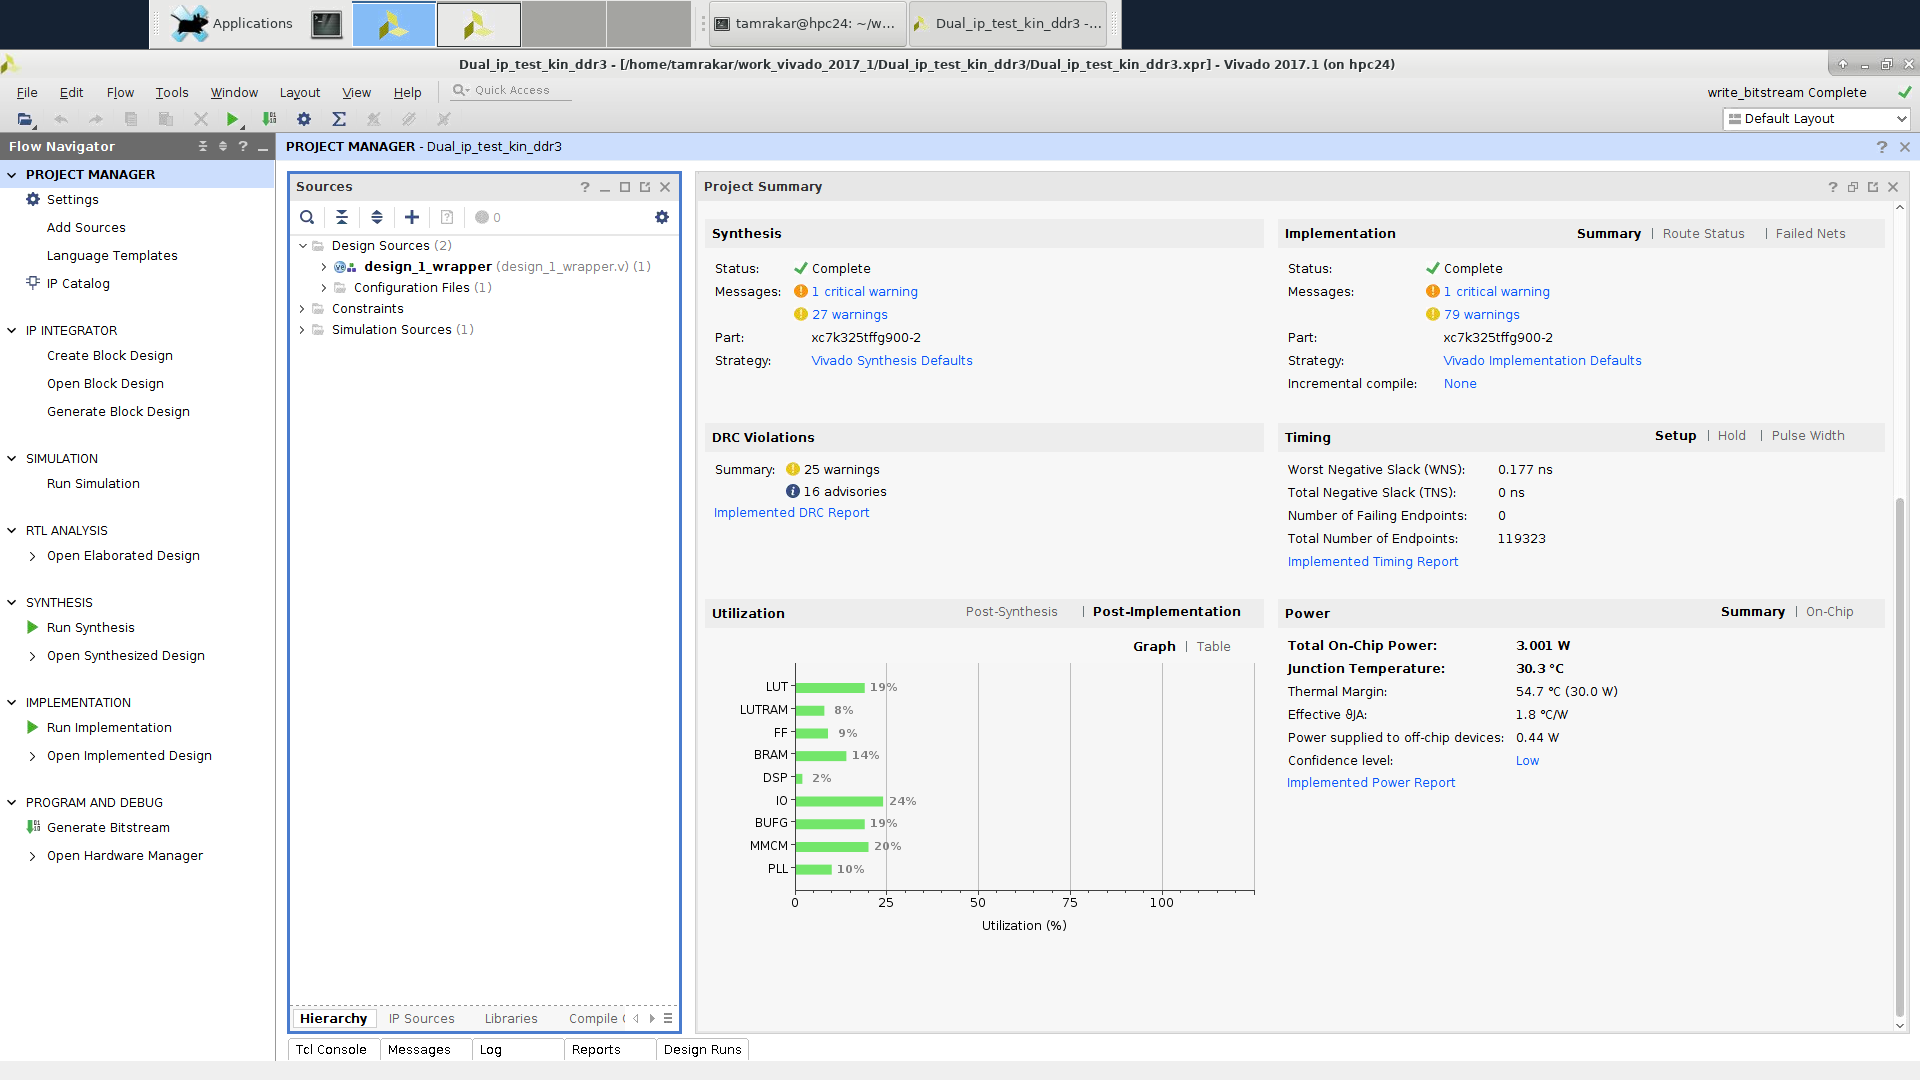
\includegraphics[width = \textwidth]{./Software/Report.png}
    \caption{IP generation report}
\end{figure}


The AXI wrapper hardware is connected to MicroBlaze and the necessary components to properly function on Kintex KC-705 Xilinx Board. A cache is attached to increase the efficiency of the executions. Following is the block-level design of the interconnections of hardware for Testing.\\



\begin{figure}[H]
    \centering
    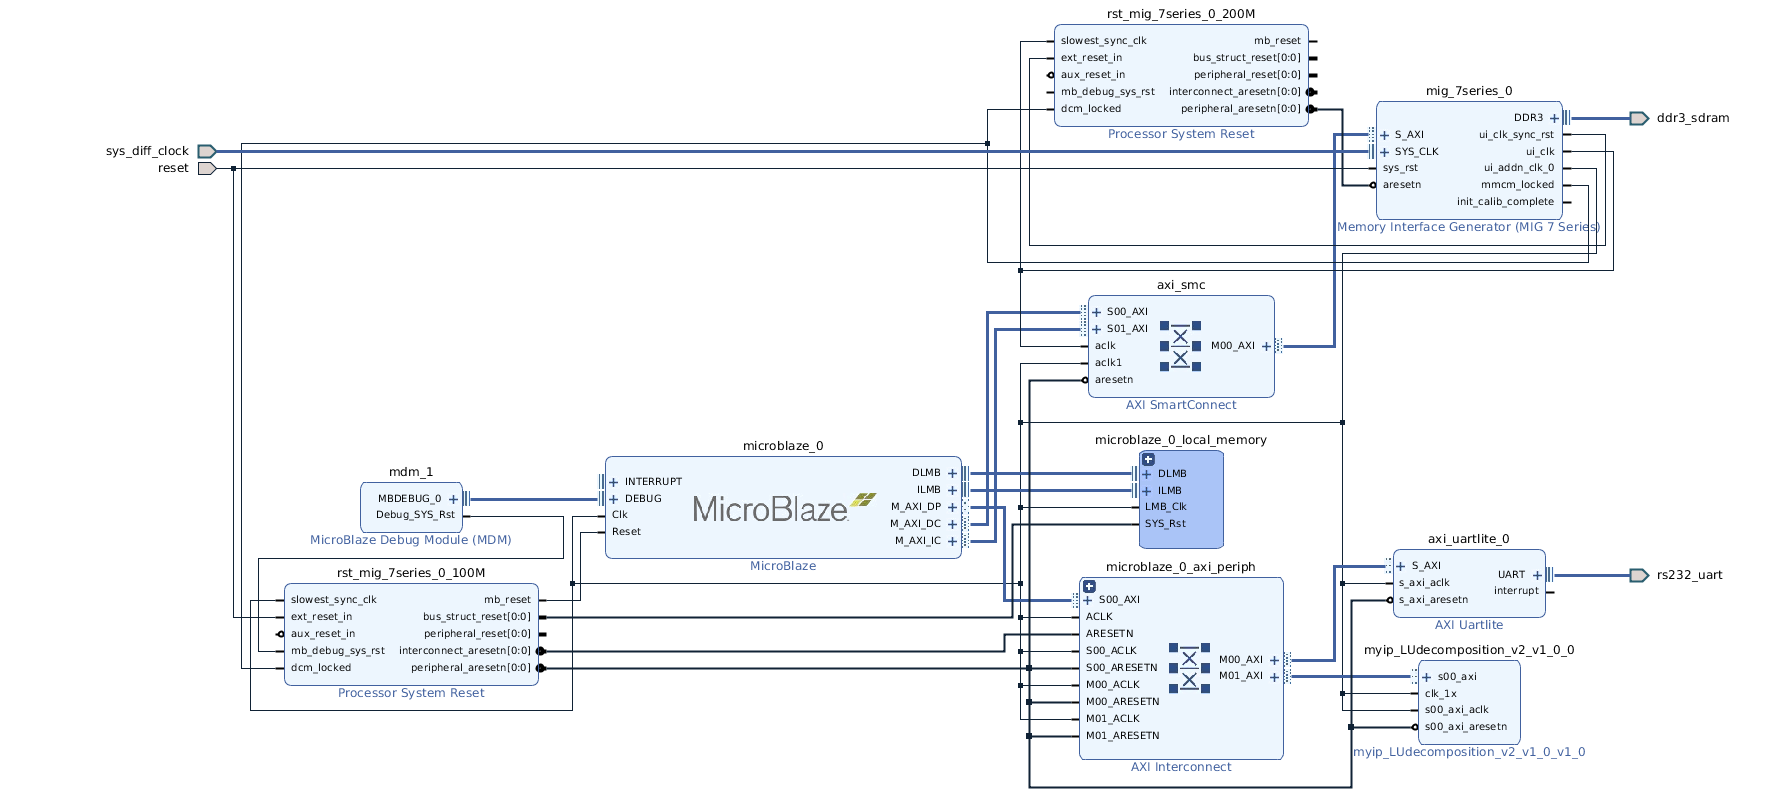
\includegraphics[width = \textwidth]{./Software/Schematic_.png}
    \caption{MicroBlaze interconnect}
\end{figure}

Microblaze code generated by the schedule for uploading instructions and data stream is used for interfacing IP and MicroBlaze. This was implemented and tested successfully on the Kintex KC-705 board, and the output is taken from UART and verified with golden reference generated by MATLAB script.
\\
\\
Shakti-based architecture Design is successfully constructed, integrated, and implemented on the Xilinx Arty-100T board. Some linguistic edition was required for ShaktiSDK because of different ISA, and accelerator tested results successfully

\begin{figure}[H]
    \centering
    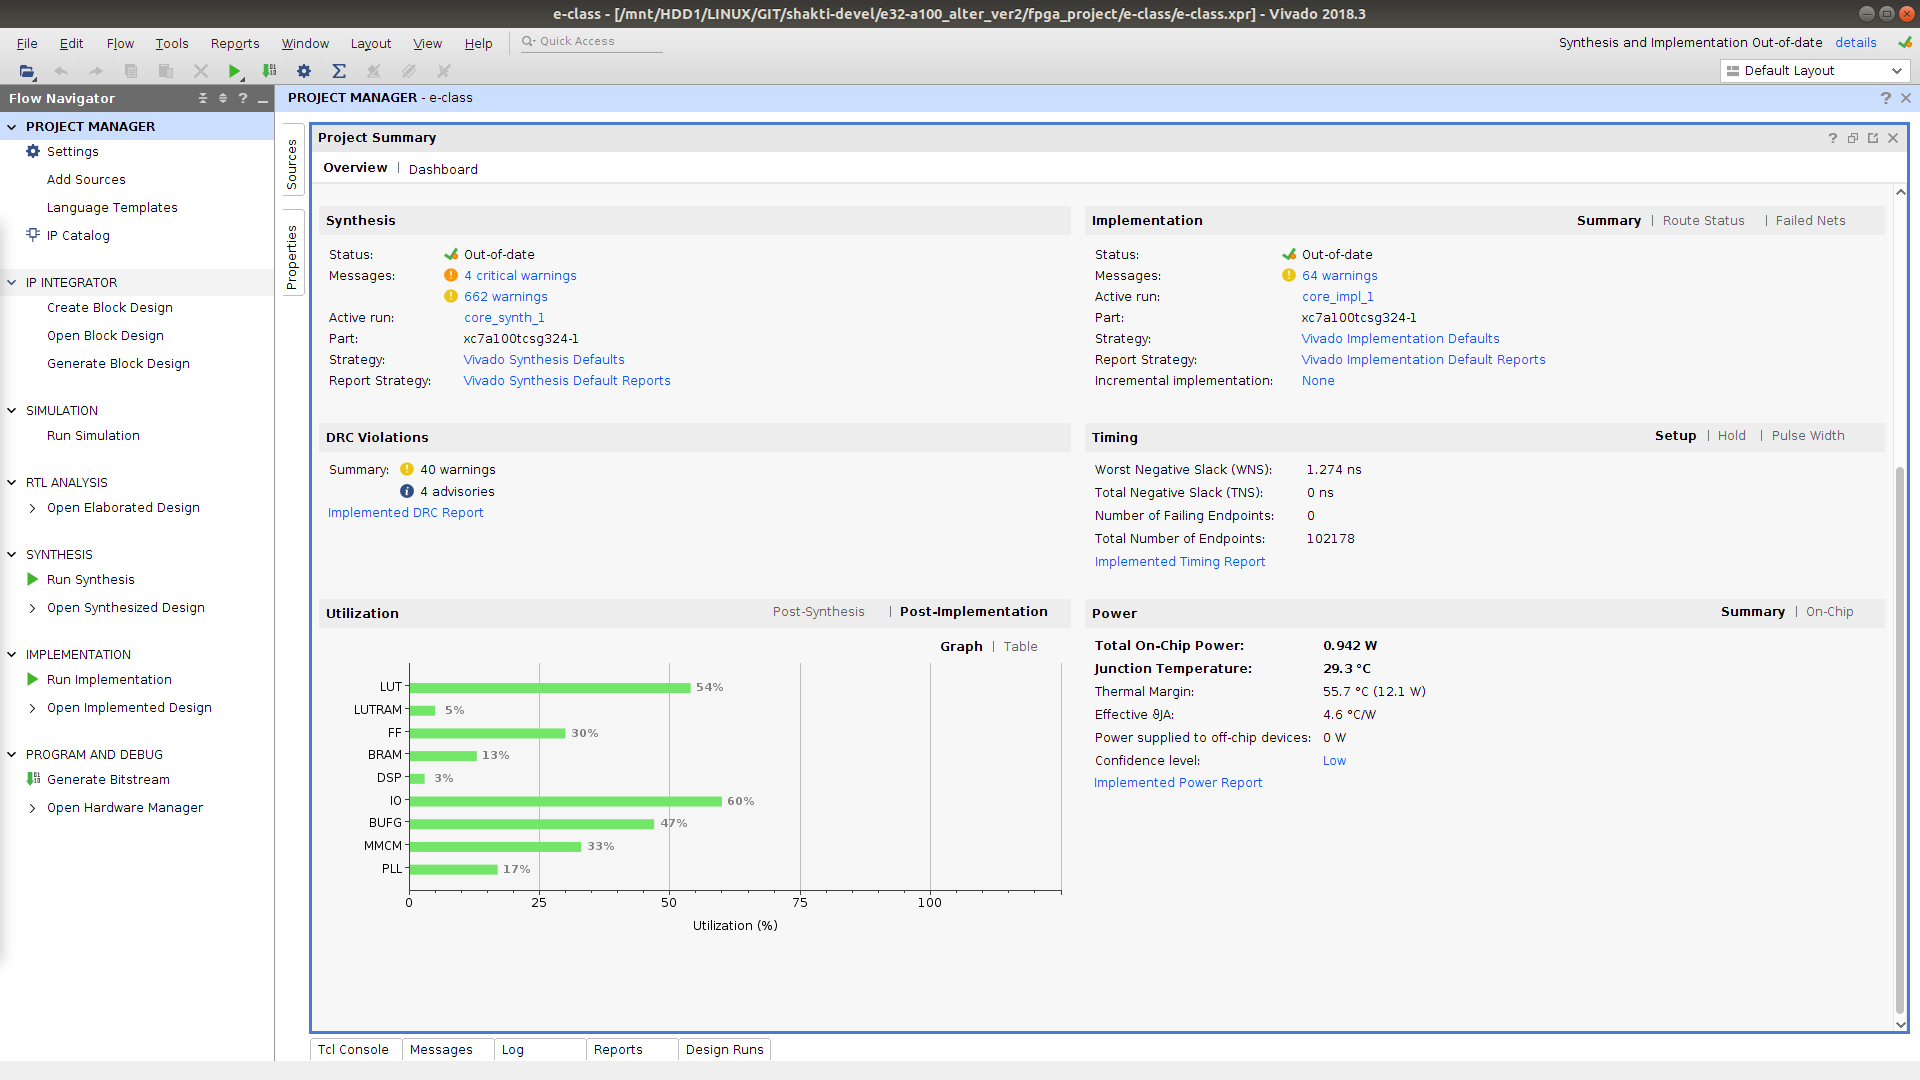
\includegraphics[width = \textwidth]{./Software/eclass.png}
    \caption{Shakti interconnect report}
\end{figure}

Accomplished final ASIC Design successfully with the help of OpenRAM( for SRAM), OpenLane(for Processing Elements), and Cadence SOC encounter( Hardening the Macros). The Proper sign-off tool decks were absent for Physical verification, although the design achieved the generic physical verification and Timing constraints.The overall Chip Area is $3796.630 \times 4944.565  \mu m^2$ i.e $ 18.772 mm^2 $

\begin{figure}[H]
    \centering
    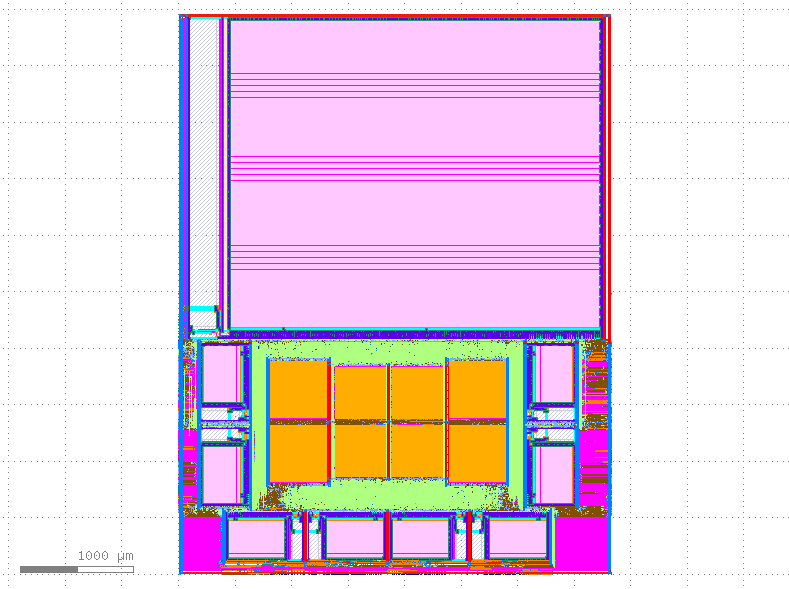
\includegraphics[width = \textwidth]{./Software/Final.png}
    \caption{ASIC Implementation with 8 SRAMs and 4 Processing Elements}
\end{figure}


Following are the scope for further improvements and implementation in the project:-
\begin{itemize}
	\item Other Scheduling Technique
	\item Other Matrix decomposition
    \item Scalable Architecture
%    \item Infallible Scheduler
\end{itemize}
